\documentclass[10pt,dvipdfmx]{standalone}
% \documentclass[10pt,dvipdfmx,b5paper,papersize]{jsarticle}
\usepackage{tikz}
\usetikzlibrary{calc}
% \usetikzlibrary{arrows.meta}
\usepackage{physics}


\begin{document}

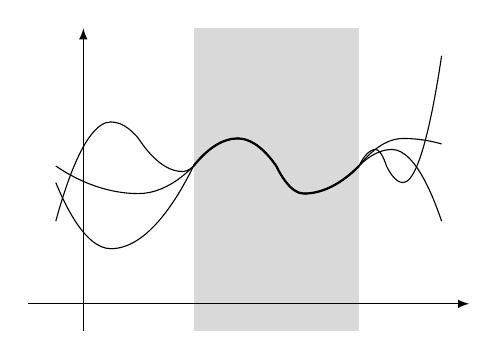
\begin{tikzpicture}[x=7mm,y=7mm,>=latex]
% \small % 文字サイズ

% gray zone
\fill[fill=gray!30] (2,0) rectangle (5,5.5);

% 座標系
\draw[->] (-1,0.5) -- (7,0.5); % x軸
\draw[->] (0,0) -- (0,5.5); % y軸
% \node(O) at (0,0) [below left]{O}; % 原点
  
% grid
% \draw[help lines] (0,0) grid (7,4);


\draw (-0.5,3) parabola bend(1,2.5) (2,3) parabola bend(2.8,3.5) (3.5,3) parabola bend(4,2.5) (5,3) parabola bend(5.8,3.5) (6.5,3.4);
\draw[] (-0.5,2) parabola bend(0.5,3.8) (1,3.5) parabola bend(1.8,2.9) (2,3) parabola bend(2.8,3.5) (3.5,3) parabola bend(4,2.5) (5,3) parabola bend(5.6,3.3) (6.5,2);
\draw[] (-0.5,2.7) parabola bend(0.5,1.5) (2,3) parabola bend(2.8,3.5) (3.5,3) parabola bend(4,2.5) (5,3) parabola bend(5.3,3.3) (5.5,3) parabola bend(5.8,2.7) (6.5,5);
\draw[thick] (2,3) parabola bend(2.8,3.5) (3.5,3) parabola bend(4,2.5) (5,3);


\end{tikzpicture}




\end{document}